% Notice how this line starts with a percent sign (%). Starting a line with a
% percent sign turns it into something called a "comment".
%
% Comments are places to put notes for people editing the LaTeX source text,
% rather than people reading the final PDF.
%
% When compiling your document into a PDF, LaTeX will ignore all comments;
% it is like they are invisible to the computer.
%
% They can also be useful if you get errors while compiling.
% If you suspect a specific line is causing problems, try turning it into a
% comment while you figure out what the problem is.
%
% Then after you fix the problem, you can "uncomment" the troublesome line:
% just removing the percent sign.

% Everything between here and \begin{document} is called the preamble.
%
% The preamble is used to set up the overall style of the document,
% perform any types of customisation you feel like, and include packages.
%
% (Packages are external collections of non-default settings. They make it
% easy to customise or extend LaTeX in specific ways.)

% Tell LaTeX what kind of document we're going to be making.
% This affects many aspects of appearance and can also limit available commands.
% For example, it isn't possible to use chapters within an article.
% Inside square brackets we provide options which switch from
% the default of letter-sized paper with 10pt font to A4 paper with 12pt font.
\documentclass[a4paper,12pt]{article}

% LaTeX doesn't know about graphics by default.
% The following extends LaTeX so that we'll be able to include images in our document.
\usepackage{graphicx}

% By default, bibliographies in LaTeX are a little unwieldy. To make
% bibliographies easier to work with, you'll usually use a package
% such as natbib:
\usepackage{natbib}

% The following package provides useful extensions such as
% an environment for aligning multiple equations on equal signs.
\usepackage{amsmath}

% A package for advanced diagram management.
\usepackage{tikz}
\usetikzlibrary{positioning}

% This package is required for \FloatBarrier (see document body).
\usepackage{placeins}

% Put hyperlinks into the document and change their default colouring.
% This will also place hyperlinks from the table of contents to the
% section headings, and between cross-references.
\usepackage[bookmarks=false, pdfstartview=FitH]{hyperref}
\hypersetup{
    colorlinks=true,
    urlcolor=blue,
    linkcolor=black,
    citecolor=black
}


% It's possible to customise LaTeX using commands in the preamble.
% Uncomment the following lines to experiment:
%\renewcommand{\theenumi}{\roman{enumi}}
%\renewcommand{\labelitemi}{***}
%
%\addtolength{\hoffset}{-1cm}
%\addtolength{\textwidth}{2\hoffset}

% Set up information for use by \maketitle.
\title{Hello world}
\author{J. Smith}
\date{} % Stop the current date from appearing in the title.


% End of preamble. Now add content.
\begin{document}

% Use information already specified in the preamble to create a title.
\maketitle

% Use information from section headings to build a TOC.
\tableofcontents


% Input LaTeX source code from other files.
\section{Introduction}

\LaTeX\ is a free, open source and cross-platform typesetting system. It was originally released in the mid-1980s by Leslie Lamport as a way of automating many aspects of Donald Knuth's \TeX\ programming language.
The word ``\LaTeX'' is a portmanteau of ``Lamport \TeX{}''.
Note that ``\TeX'' is from the Greek word $\tau\epsilon\chi\nu\eta$, pronounced "techneh";
thus, \LaTeX\ should be pronounced ``Lah-Tech'' or ``Lay-Tech'', never ``lateks''.

Note that in \LaTeX\ it looks kind of ugly to use the standard "double-quotation mark".
It looks better to write backwards-apostrophes with a backtick (\texttt{`}).
If you want double quotation marks, use two backticks on the left and two apostrophes on the right like so:

\begin{verbatim}
The word ``\LaTeX'' is a portmanteau of ``Lamport \TeX{}''.
\end{verbatim}

A simple equation describes the curvature of spacetime due to mass and energy:

\begin{equation}
    R_{\mu \nu} - {1 \over 2}g_{\mu \nu}\,R + g_{\mu \nu} \Lambda = {8 \pi G \over c^4} T_{\mu \nu}\label{eq:einstein-field-equations}
\end{equation}

\section{Cat pictures}
\label{sec:cats}
% Labelling a section lets us refer to it from other places in the document.

Cat pictures are a great teaching aid \citep{smith2016}. % A parenthesised citation.

\citet{smith2016} says every \LaTeX\ presentation should begin with a cat picture. % An in-text citation.

Use a command provided by graphicx to add a picture:

\includegraphics{figures/cat.jpg}

Use an option in square brackets to change the image width:

\includegraphics[width=0.9\textwidth]{figures/cat.jpg}

Note that Figure~\ref{fig:cat-picture-1} is inside a figure environment
defined like so:

\begin{verbatim}
\begin{figure}
    \begin{center}
        \includegraphics{figures/cat.jpg}
        \caption{Meow!}
        \label{fig:cat-picture-1}
    \end{center}
\end{figure}
\end{verbatim}

This lets LaTeX float the image to a spot where it will look reasonably tidy.

At first this can take some getting used to because the figure in the final
PDF will often not appear right where you specify it in the \LaTeX\ source.
In fact, if you have it set in your mind that an image
must appear at an exact point you specify, \LaTeX\ will
seem wilfully frustrating.
People can get quite irate when they think they know how their document
should look, only to find that \LaTeX\ stubbornly disagrees.

To avoid frustration, try to train yourself to trust
that \LaTeX\ knows what it's doing.
It was, after all, written with beautiful typesetting as its highest priority.
To stick to best practice, put each image inside a figure environment,
with a label, and then rather than saying ``see the following image:'',
say ``see Figure~\ref{fig:cat-picture-1}''.

\begin{figure}
    \begin{center}
        \includegraphics{figures/cat.jpg}
        \caption{Meow!}
        \label{fig:cat-picture-1}
    \end{center}
\end{figure}

Note that other types of floating environments are available, such as for tables.

Also note that when including mathematical or technical diagrams,
it's often prettier and easier to manage if you create them
directly in your \LaTeX\ document rather than including a pre-rendered image.

\begin{figure}
    \begin{center}
        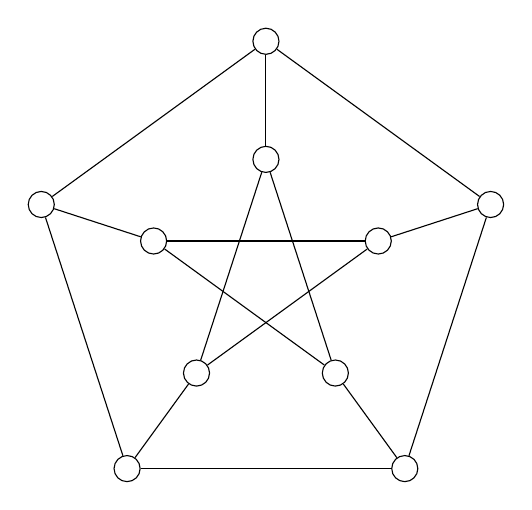
\begin{tikzpicture}
            \node (inner1) at (90:1.5) [shape=circle,draw] {};
            \node (inner2) at (162:1.5) [shape=circle,draw] {};
            \node (inner3) at (234:1.5) [shape=circle,draw] {};
            \node (inner4) at (306:1.5) [shape=circle,draw] {};
            \node (inner5) at (18:1.5) [shape=circle,draw] {};
            \node (outer1) at (90:3) [shape=circle,draw] {};
            \node (outer2) at (162:3) [shape=circle,draw] {};
            \node (outer3) at (234:3) [shape=circle,draw] {};
            \node (outer4) at (306:3) [shape=circle,draw] {};
            \node (outer5) at (18:3) [shape=circle,draw] {};
            \draw (inner1)--(inner3);
            \draw (inner1)--(inner4);
            \draw (inner2)--(inner4);
            \draw (inner2)--(inner5);
            \draw (inner3)--(inner5);
            \draw (inner1)--(outer1);
            \draw (inner2)--(outer2);
            \draw (inner3)--(outer3);
            \draw (inner4)--(outer4);
            \draw (inner5)--(outer5);
            \draw (outer1)--(outer2);
            \draw (outer2)--(outer3);
            \draw (outer3)--(outer4);
            \draw (outer4)--(outer5);
            \draw (outer5)--(outer1);
        \end{tikzpicture}
        \caption{Petersen graph}
        \label{fig:petersen}
    \end{center}
\end{figure}

Figure~\ref{fig:petersen} requires you to use tikz-pgf
\citep{tantau-tikz-pgf-3.0.1a}.
This is a general purpose package for drawing diagrams
within a \LaTeX\ document.
There are also packages specifically for things like
commutative diagrams, Feynman diagrams, and musical scores.
However, tikz is general purpose, powerful, and widespread enough
that it will cover most scenarios.

\section{Lists}

Ordered:
\begin{enumerate}
  \item The First
  \item The Second
\end{enumerate}

Unordered:
\begin{itemize}
  \item Some point
  \item Another point
\end{itemize}

\section{Formatting text and mathematics}\label{sec:formatting}

The following will explore some of the text formatting commands often used in
\LaTeX.

\emph{This text is emphasised.}

\textit{This text also looks emphasised because it's in italics,
    but if we now use the emph command inside italics,
\emph{it will switch italics off}.}

\textbf{This text is bolded.}

\textsc{Small-caps is useful if you want to sound like Death
from a Terry Pratchett book.}

To enter mathematics, we already saw one method in
Equation~\ref{eq:einstein-field-equations}.
You can also write equations in-line (i.e. as part of surrounding text)
using dollar signs like so: $e^{i\pi} - 1 = 0$.
Another option more concise than the equation environment
is to use double dollar signs:

$$R_{\mu \nu} - {1 \over 2}g_{\mu \nu}\,R + g_{\mu \nu} \Lambda = {8 \pi G \over c^4} T_{\mu \nu}$$

Notice how using double dollar signs suppresses the equation numbering.

Often we want multiple lines of working aligned on equals signs.
There are two ways to do this.
Built in to \LaTeX\ is the eqnarray environment.
For example, to specify a Kermack-McKendrick SIR epidemic model, you can write:

\begin{verbatim}
\begin{eqnarray}
    \dot{S}	&=&	-\beta{S}I\\
    \dot{I}	&=&	\beta{S}I-\gamma{I}\\
    \dot{R}	&=&	\gamma{I}
\end{eqnarray}
\end{verbatim}

Each double-backslash starts a new line; ampersands delimit ``columns''.
This turns into:

\begin{eqnarray}
    \dot{S}	&=&	-\beta{S}I\\
    \dot{I}	&=&	\beta{S}I-\gamma{I}\\
    \dot{R}	&=&	\gamma{I}
\end{eqnarray}

Note that this notation of columns delimited by ampersands,
and lines separated by double-backslashes,
is used in other contexts in LaTeX, such as when entering tables.

There is also a starred version of eqnarray, which suppresses numbering:

\begin{verbatim}
\begin{eqnarray*}
    \dot{S}	&=& -\beta{S}I\\
    \dot{I}	&=& \beta{S}I-\gamma{I}\\
    \dot{R}	&=& \gamma{I}
\end{eqnarray*}
\end{verbatim}

\begin{eqnarray*}
    \dot{S}	&=& -\beta{S}I\\
    \dot{I}	&=& \beta{S}I-\gamma{I}\\
    \dot{R}	&=& \gamma{I}
\end{eqnarray*}

Many people prefer to use the align environment provided by the amsmath package,
which only requires one equals sign:

\begin{verbatim}
\begin{align*}
    \dot{S}	&= -\beta{S}I\\
    \dot{I}	&= \beta{S}I-\gamma{I}\\
    \dot{R}	&= \gamma{I}
\end{align*}
\end{verbatim}

\begin{align*}
    \dot{S}	&= -\beta{S}I\\
    \dot{I}	&= \beta{S}I-\gamma{I}\\
    \dot{R}	&= \gamma{I}
\end{align*}

\section*{Sectioning}

\LaTeX\ allows the following sectioning commands:

\begin{verbatim}
\part{}
\chapter{}
\section{}
\subsection{}
\subsubsection{}
\paragraph{}
\subparagraph{}
\end{verbatim}

Not all sectioning types are available in all document classes.
You probably won't use part, paragraph or subparagraph very often (or ever).

For an article you'll usually only need section and subsection.
If you need chapter (for example, in a thesis), you'll probably use
the report document class.

Note that this unnumbered section was created using an asterisked (``starred'')
sectioning command, like so:

\begin{verbatim}
\section*{Sectioning}
\end{verbatim}

Starred sections not only have their numbering suppressed but also will not
appear in the table of contents.
Go and check, you'll see that the current section isn't mentioned.

\section{Other odds and ends}

\subsection{More on floats}

Recall in Section~\ref{sec:cats} that there are other types of floats,
such as for tables; furthermore, Section~\ref{sec:formatting}
mentioned that ampersands and double-backslashes are used when
describing tables.
Table~\ref{tab:example-table-1} provides an example.

\begin{table}
    \begin{center}
        \begin{tabular}{l|r@{.}l|r}
            Animals & \multicolumn{2}{|c|}{Numbers} & Names \\
            \hline\hline
            Cat     &    1&2                        & Jane  \\
            Dog     &   12&34                       & John  \\
            Rabbit  &  123&456                      & Jessica
        \end{tabular}
        \caption{Some silly table.}
        \label{tab:example-table-1}
    \end{center}
\end{table}

When using floating environments such as figures and tables,
you'll often want to make sure LaTeX doesn't float them into the next section.
When finishing a section, you can force LaTeX to flush out any remaining
floats before starting the next section using the following command:

\begin{verbatim}
\FloatBarrier
\end{verbatim}

\FloatBarrier


\subsection{Defining your own commands}

\LaTeX\ is very customisable.
One thing you can do is create ``macros'',
shortcuts for longer commands if you get tired of
typing out the same thing over and over.

In your preamble, try putting:

\begin{verbatim}
\newcommand{\incgr}[1]{\includegraphics{#1}}
\end{verbatim}

You can now include images by writing:

\begin{verbatim}
\incgr{figures/cat.jpg}
\end{verbatim}

To redefine an existing command, use ``\\renewcommand''.

Since \LaTeX handles many aspects of typesetting by creating hidden commands,
\\renewcommand is often used to customise page styling.
For example, to reduce the margin width put the following in your preamble:

\begin{verbatim}
\addtolength{\hoffset}{-1cm}
\addtolength{\textwidth}{2\hoffset}
\end{verbatim}


\subsection{\LaTeX\ and version control}

Since \LaTeX\ source files are written in plain text,
they are very amenable to version control using systems such
as Subversion, Mercurial, and Git.

This has many benefits.
At a minimum, version control will keep a history of changes in your document,
and allow you to easily collaborate with others.

Depending on which type of version control you use, there could be other benefits.
In particular, if you use Git,
you'll usually have copies of your \LaTeX\ project
synchronised between all your machines.
In this case, if one computer has a malfunction,
you've automatically got multiple backups available.

Secondly, Git makes it fast and easy to create branches within your project.
One possible benefit of this is that you could create a new branch for
each journal you submit an article to.
Another possibility is to have a ``supervisor'' branch
where you can experiment with suggestions made by your supervisor.
Assuming you disagree with your supervisor
(pfft, what would they know, righ?),
you can quickly revert back to the master branch.

If you want to version control your \LaTeX\ documents,
a good practice is to put line breaks after each major use of punctuation,
especially at each new sentence.
The reason for doing it this way is that Git uses 
line breaks to help it find differences between documents.

If you have each entire paragraph all on one line,
changes to any word in the paragraph will show up as changes
in the entire paragraph.
When looking at the difference between two versions,
seeing that a whole paragraph has changed is less useful
than seeing that a particular sentence or phrase has changed.

More information on this topic is available at
\citet{stackoverflow-git+latex-workflow},
\citet{tex-stackexchange-git-latex-and-branches-workflow},
and \citet{allen-collaborating-with-latex-and-git}.

For more information on how to use Git, see
\citet{gonzalez-huang-swc-git-novice} for introductory
material used by \href{http://www.software-carpentry.org}{Software Carpentry},
or \citet{chacon-pro-git-2014} for a more comprehensive reference.


\subsection{Guides and extra help}

Since \LaTeX\ is free and open source, there is a great deal
of online material available in the form of guides, tutorials,
technical package documentation,
and question-answer sites where people discuss problems they're having.

Almost always, anything you're having trouble with or want to know
more about has already been discussed a thousand times elsewhere.
So, whenever you are having trouble, your first port of call should usually
be your preferred search engine in your chosen web browser.

\citet{oetiker-lshort-2015} (usually referred to as ``lshort'')
gives a comprehensive and readable introduction to \LaTeX.
Everyone who uses \LaTeX, whether novice or advanced,
will usually keep a copy of lshort handy.
There is another extensive introductory survey of \LaTeX\ on
\href{https://en.wikibooks.org/wiki/LaTeX}{Wikibooks}.

When using \textsc{Bib}\TeX, it's a good idea to keep \citet{patashnik-bibtex-1988}
close by, as it lists all the available citation types and their
required vs optional fields.
Other useful references are in \citet{markey-ttb-2009}
and \citet{daly-natbib-2010}.

If you're going to use \LaTeX\ a lot, \citet{mittelbach-goossens-2004}
is a very comprehensive text with just about everything you can think of,
including discussions of a wide variety of packages,
and instructions on how to customise all aspects of the document,
as well as how to roll your own classes and packages.

If you want to know more about how \LaTeX\ works under the hood,
a complete introduction to plain \TeX\ appears in \citet{knuth-texbook-1986}.

If you'd like more in-person help,
\href{http://melbourne.resbaz.edu.au/}{Research Bazaar}
runs a free weekly drop-in session for postgrads and early career researchers
called ``Hacky Hour''.
This happens 3pm every Thursday at \href{http://tsububar.com.au/}{Tsubu Bar}.




% Specify what style the bibliography should follow.
\bibliographystyle{plainnat}

% Specify which file contains the bibliography data.
% This is a file with a ".bib" extension, in this case "main.bib".
% Notice how it's not necessary to specify the extension in the following command:
\bibliography{main}
\end{document}
